\documentclass[11pt]{sdm}
\usepackage{xcolor}
\usepackage{hyperref}
\definecolor{default-linkcolor}{HTML}{A50000}
\definecolor{default-filecolor}{HTML}{A50000}
\definecolor{default-citecolor}{HTML}{A50000}
\definecolor{default-urlcolor}{HTML}{A50000}
\hypersetup{
    colorlinks=true,
    linkcolor=default-linkcolor,
    filecolor=default-filecolor,
    citecolor=default-citecolor,
    urlcolor=default-urlcolor,
    breaklinks=true,
    pdftitle={Function placement for FaaS applications in the fog},
    pdfauthor={Volodia PAROL-GUARINO},
    pdflang={en},
    pdfpagemode=FullScreen,
    }
    
\usepackage{amsmath,amssymb,amsfonts}
\usepackage{algorithmic}
\usepackage{graphicx}
\usepackage{textcomp}
\usepackage{xstring}
\usepackage[inline, shortlabels]{enumitem}
\usepackage[acronym]{glossaries}
\usepackage[backend=bibtex,style=ieee,natbib=true]{biblatex}
\usepackage{utf8}
\usepackage{lscape} 

\usepackage{diagbox} %table split headers
\usepackage{longtable}
\usepackage{array}
\usepackage{rotating}
\usepackage{eqparbox}
\usepackage{makecell, caption, booktabs}


\DeclareNameFormat{labelname:poss}{% Based on labelname from biblatex.def
  \nameparts{#1}% Not needed if using Biblatex 3.4
  \ifcase\value{uniquename}%
    \usebibmacro{name:family}{\namepartfamily}{\namepartgiven}{\namepartprefix}{\namepartsuffix}%
  \or
    \ifuseprefix
      {\usebibmacro{name:first-last}{\namepartfamily}{\namepartgiveni}{\namepartprefix}{\namepartsuffixi}}
      {\usebibmacro{name:first-last}{\namepartfamily}{\namepartgiveni}{\namepartprefixi}{\namepartsuffixi}}%
  \or
    \usebibmacro{name:first-last}{\namepartfamily}{\namepartgiven}{\namepartprefix}{\namepartsuffix}%
  \fi
  \usebibmacro{name:andothers}%
  \ifnumequal{\value{listcount}}{\value{liststop}}{'s}{}}
\DeclareFieldFormat{shorthand:poss}{%
  \ifnameundef{labelname}{#1's}{#1}}
\DeclareFieldFormat{citetitle:poss}{\mkbibemph{#1}'s}
\DeclareFieldFormat{label:poss}{#1's}
\newrobustcmd*{\citepossalias}{%
  \AtNextCite{%
    \DeclareNameAlias{labelname}{labelname:poss}%
    \DeclareFieldAlias{shorthand}{shorthand:poss}%
    \DeclareFieldAlias{citetitle}{citetitle:poss}%
    \DeclareFieldAlias{label}{label:poss}}}
\newrobustcmd*{\citeposs}{%
  \citepossalias%
  \textcite}
\newrobustcmd*{\Citeposs}{\bibsentence\citeposs}
\newrobustcmd*{\citeposss}{%
  \citepossalias%
  \textcites}

\addbibresource{biblio.bib} %added
\def\BibTeX{{\rm B\kern-.05em{\sc i\kern-.025em b}\kern-.08em
    T\kern-.1667em\lower.7ex\hbox{E}\kern-.125emX}}

%numeroter les pages
\pagestyle{plain}

\title{Function placement for FaaS applications in the fog}
\author{Volodia \textsc{Parol-Guarino}}
\supervisorOne{Nikolaos \textsc{Parlavantzas}}
\supervisorTwo{First\_Name \textsc{Name} of your second supervisor}
\team{MYRIADS}
%One of:
% ens-Rennes  esir    insa-rennes   rennes1  
% enssat    logoUbs   tsupelec
%here rennes1 for example
\school{insa-rennes}


% the domain should be one or two of:
% Technology for Human Learning 
% Artificial Intelligence 
% Computer Arithmetic
% Hardware Architecture
% Automatic Control Engineering
% Bioinformatics 
% Biotechnology
% Computational Complexity 
% Computational Engineering, Finance, and Science
% Computational Geometry 
% Computation and Language 
% Cryptography and Security 
% Computer Vision and Pattern Recognition
% Computers and Society 
% Databases 
% Distributed, Parallel, and Cluster Computing 
% Digital Libraries
% Discrete Mathematics 
% Data Structures and Algorithms 
% Embedded Systems 
% Emerging Technologies 
% Formal Languages and Automata Theory 
% General Literature 
% Graphics 
% Computer Science and Game Theory 
% Human-Computer Interaction 
% Computer Aided Engineering 
% Medical Imaging 
% Information Retrieval 
% Information Theory 
% Ubiquitous Computing 
% Machine Learning
% Logic in Computer Science 
% Multiagent Systems 
% Mobile Computing
% Multimedia
% Modeling and Simulation 
% Mathematical Software 
% Numerical Analysis 
% Neural and Evolutionary Computing 
% Networking and Internet Architecture 
% Operating Systems 
% Performance 
% Programming Languages 
% Robotics 
% Operations Research
% Symbolic Computation 
% Sound
% Software Engineering 
% Social and Information Networks 
% Systems and Control 
% Image Processing 
% Signal and Image Processing 
% Document and Text Processing
% Web
\domain{Domain:  Distributed, Parallel, and Cluster Computing -- Fog: Cloud after the edge}

%write your abstract here
\abstract{write your abstract here}


\makeglossaries   
\newacronym{FaaS}{FaaS}{Function-as-a-Service}
\newacronym{OSS}{OSS}{Open-Source Software}
\newacronym{AI}{AI}{Artificial Intelligence}
\newacronym{SLA}{SLA}{Service Level Agreement}
\newacronym{SLO}{SLO}{Service Level Objectives}
\newacronym{VM}{VM}{Virtual Machine}
\newacronym{PAPS}{PAPS}{Partitioning, Allocation, Placement, and Scal-
ing}
\newacronym{IoT}{IoT}{Internet of Things}
\newacronym{SEP}{SEP}{Serverless Edge Platform}
\newacronym{IoV}{IoV}{Internet of Vehicules}
\newacronym{RSU}{RSU}{Road-Side Unit}
\newacronym{VCG}{VCG}{Vickrey-Clarke-Groves}
\newacronym{SDN}{SDN}{Software-Defined Networking}
\newacronym{LI}{LI}{Least-Impedance}
\newacronym{RP}{RP}{Random-Proportional}
\newacronym{RR}{RR}{Round-Robin}
\newacronym{LaSS}{LaSS}{LAtency Sensitive Serverless}
\newacronym{LLA}{LLA}{Low Latency Application}
\newacronym{QoS}{Qos}{Quality-of-Service}    
\newacronym{MEC}{MEC}{Multi-access Edge Computing}
\newacronym{ACO}{ACO}{Ant Colony Optimization}
\newacronym{ETSI}{ETSI}{European Telecommunications Standards Institute}
\newacronym{NFV}{NFV}{Network Function Virtualization}
\newacronym{GPU}{GPU}{Graphical Processing Unit}
\newacronym{QoE}{QoE}{Quality of Experience}
\newacronym{SoC}{SoC}{System-on-a-Chip}

\begin{document}
\maketitle

%*****************************************************************%

\section{Introduction}
\begin{itemize}
	\item Introduce \gls{FaaS} paradigm (as an extension of serverless?)
 	\item Serverless is still improving, especially on the biggest problems (eg. coldstart) where even the base technologies are starting to be questioned and concurrenced by faster and more precise technologies \citet{hykes_solomon_2019}
    \item Introduce Fog, along with a word about \gls{MEC} and cloudlets
    \item indicated sections where to find more details
    \item {List of open questions from \citet{kjorveziroski_iot_2021}
    \begin{enumerate}
        \item Scheduling
        \item deployement
        \item performance
        \item cold start
        \item vendor lock-in
        \item security \& isolation
        \item improvement to function chaining / combination (preferrably even)
        \item support for hardware acceleration (GPU, AI)
    \end{enumerate}
    \item { Another approach is contributed by \citet{xie_when_2021}. They explore the challenges from the perspective of networking, as this is the main layer that enables the Fog to exist in the first place. It is relevant because of \gls{NFV} and \gls{SDN} and the relative closeness of \gls{MEC}
    \begin{enumerate}
        \item service deployement
        \item resource awareness and service discovery
        \item service scheduling
        \item incentive mechanism
        \item exceptions and failure recovery
    \end{enumerate}
    }
    \item Usually papers about IoT because these kind of devices are expected to take over
    \item Research on the metrics to optimize as well as the way to optimize them
    \item This issue is a problem because strategies needs to precisely account for this such as \citeposs{kaffes_centralized_2019} work that emphasizes about predictabability of performances. To do so they defend a centralized approaches instead of decentralization. Main causes: burstiness of the load + cold start that need to be managed and orchestrated at a higher level
    \item cold-start also a problem, especially in a constrained Fog node.
    \item Need to introduce to the ``big question''. Where to place \gls{FaaS} in the Fog, in a place that spans from the emitter to the cloud itself, while traveling a number of heterogeneous nodes.
    \item Explain in what it is difficult to solve (heterogeneity, dynamism, ownership, geographical distributions, etc.)
    }

    
\end{itemize}

\section{Background}

Four concepts currently coexists. One defines Fog. They all share a same basis of both benefits and challenges of developing and utilizing the Edge -- and beyond \cite{george_nanolambda_2020}.

\begin{description}
	\item[Edge Computing] defines the utilization of computing resources located at the edge of networks. The user (event producer) is far from the core/Cloud in the Cloud-centered model. Having access to resources closer to the user could alleviate latencies and ameliorate both \gls{QoS} and \gls{QoE} of applications. When referring to Edge Computing, it is exclusively resources located at the edge that are targeted.
		
	\item[Cloudlets] first appeared in \cite{satyanarayanan_case_2009} in \citedate{satyanarayanan_case_2009}. The metaphor is to move a part of the cloud as close to the user as possible, eg. service it in the wireless LAN he is connected to. In this architecture, the mobile user exploits a \gls{VM} quickly instantiated on demand. It allows him to utilize a trusted, resource-rich computer -- or cluster of computers. This computer -- a mobility enhanced small-scale cloud data center located at the edge -- is required to be ``well-connected'' to the Internet and available for use by nearby mobile devices. As cloudlets are distributed geographically, one great preoccupation has been how to deal with the \gls{VM} instances as the mobile user changes location.
	
	\item[\acrfull{MEC}] was first introduced as \emph{Mobile} Edge Computing. It was born as a standardization from Huawei, IBM, Intel, Nokia Networks, NTT DoCoMo, Vodafone, and other companies. Their efforts lead to a new \gls{ETSI} standard. The name change occurred to bring the attention on the relevance of the technology for all the networks -- and not only the radio-based ones such as 5G. The standard is a way to unite both the telco an IT-Cloud worlds \cite{dahmen-lhuissier_etsi_nodate-1}. The specification enables applications to be hosted in a multi-vendor, multi-access, edge-only computing environment -- ``on-top'' of the mobile network elements. This is enabled by other emerging technologies such as \gls{NFV} \footnote{\acrfull{NFV} is the ability for networking equipment to rely on software functions rather than hardware ones \cite{redhat_what_2019}. Leveraging agility. Use cases include DHCP, firewall, and general execution of routing components, all virtualized.} and \gls{SDN} \footnote{\acrfull{SDN} dynamically routes requests in a centralized fashion. It separates the control plane from the data plane, thus sailing away from classical routing where all nodes participate in both decision making and data handling \cite{redhat_what_2019}. Centralization helps to achieve optimal routing, especially at the scale of a network operator.}. \gls{MEC} is proposed as a vertical solution for \gls{IoT} and mission critical solutions. \gls{MEC} applications also leverage virtualization to be purely software byproducts. The virtual infrastructure also includes a data plane for routing among all the connected networks: applications, internal and external. A gateway decides whether a request is granted or not. If it is, the accepted request is forwarded to the orchestrator for further processing. \gls{MEC} works in a centralized way arranged around the orchestrator. It knows the topology, available resources and \gls{MEC} services. It is planned \gls{MEC} physical nodes would be placed at edges of a telco operator's network, eg. at 5G base stations.
	
	\item[Fog computing] or Fog is a horizontally distributed architecture aiming to bring both the data plane and the control plane closer to the end-user -- the event producer -- by exploiting all the computing-enabled along the cloud-to-things continuum. Fog creates an immersive distribution of computing, where task execution occur geographically near the producer, while keeping centralized-dependent processes treated in the Cloud, where it is best handled. Fog is different from the two others edge-only approaches as it provides tools for distributing, orchestrating, managing and securing both resources and services across networks and devices living in the continuum.
	
	A Fog node has multiple functions, including but not limited to: networking, computing, accelerating (using \gls{GPU}, etc.), storing and control. It can be worked as a mesh. Fog nodes are not conceived to be present at the teclo's operator Edge in the first place, in contradiction to the \gls{MEC} model. They can be positioned between the Edge and the Cloud and event after the Edge in smaller -- maybe private -- networks.
	
	\begin{figure}[t]
		\centering
		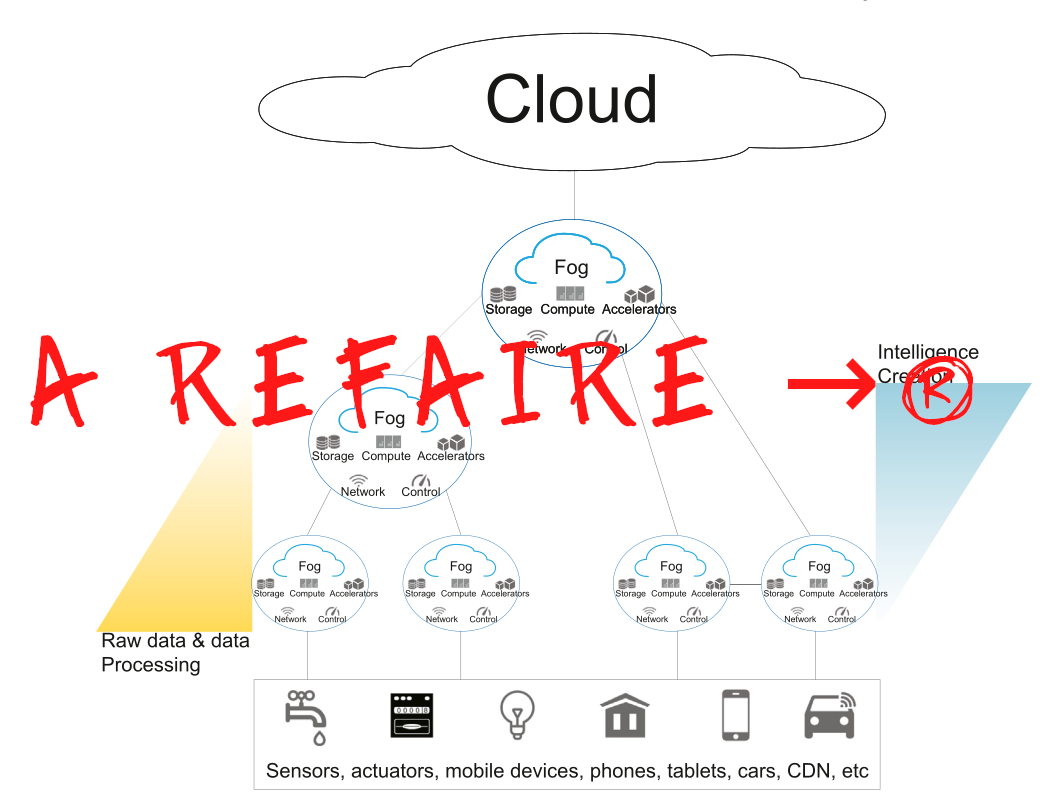
\includegraphics[width=0.75\textwidth]{./assets/FogArchi.png}
		\caption{A typical intelligence creation, hierarchical, architecture based on Fog computing}
		\label{fig:fog_archi}
	\end{figure}
	
	Fog also presents a hierarchical organization. Fog nodes at the very edge will usually be lighter on processing capabilities and may be reserved to light tasks, such as filtering or simple transformations. Getting closer to the Cloud, the value of the processing of each node will increase, as the intelligence creation will. A typical architecture is presented in \ref{fig:fog_archi}.
	
	Fog is also shown to be more energy-efficient than processing all data centrally in the Cloud \cite{ai_edge_2018}.
	
	Fog answers to a number of challenges posed by the Cloud and current models \cite{chiang_fog_2016}: 
	\begin{enumerate*}[(a)]
		\item \emph{low/deterministic latency requirements} for real time applications
		\item \emph{network bandwidth constraints} that cannot be relieved
		\item \emph{resource-constrained} producers not able to process locally
		\item \emph{uninterrupted service} with or without interruption scheduled
		\item \emph{security}, switch away from perimeter-based approaches to protecting a large number of devices, constrained, trusted or not, all without disruptions
	\end{enumerate*}
	
	Fog was first introduced by Cisco in \citeposs{bonomi_fog_2012} paper published in \citedate{bonomi_fog_2012}. They define the characteristics of Fog, in order:
	\begin{enumerate*}[(i)]
		\item low-latency and location awareness
		\item wide-spread geographical distribution
		\item mobility
		\item very large number of nodes
		\item dominance of Wireless access
		\item Real-time and streaming applications as first citizens
		\item heterogeneity
	\end{enumerate*}
	The Fog initiative is now ported by the OpenFog Consortium  \cite{ieee_standards_association_ieee_2018} constituted of ARM, Cisco, Dell, Intel, Microsoft and Princeton University \cite{chiang_fog_2016}.
\end{description}

The benefits are similar for all the paradigms, we will concentrate on Fog as it is the main topic in this report. \citet{ahmed_fog_2019} identifies key aspects that it provides:
\begin{enumerate*}[(a)]
	\item latency reduction
	\item bandwitdh optimization
	\item computational offloading
	\item Privacy and security through on-premise exploitation
	\item Service management as a middleware
	\item edge-device monitoring
	\item Energy efficiency-enabling vector
	\item Cost savings through plateform aquisition
	\item Content caching
\end{enumerate*}.


\begin{figure}[t]
	\centering
	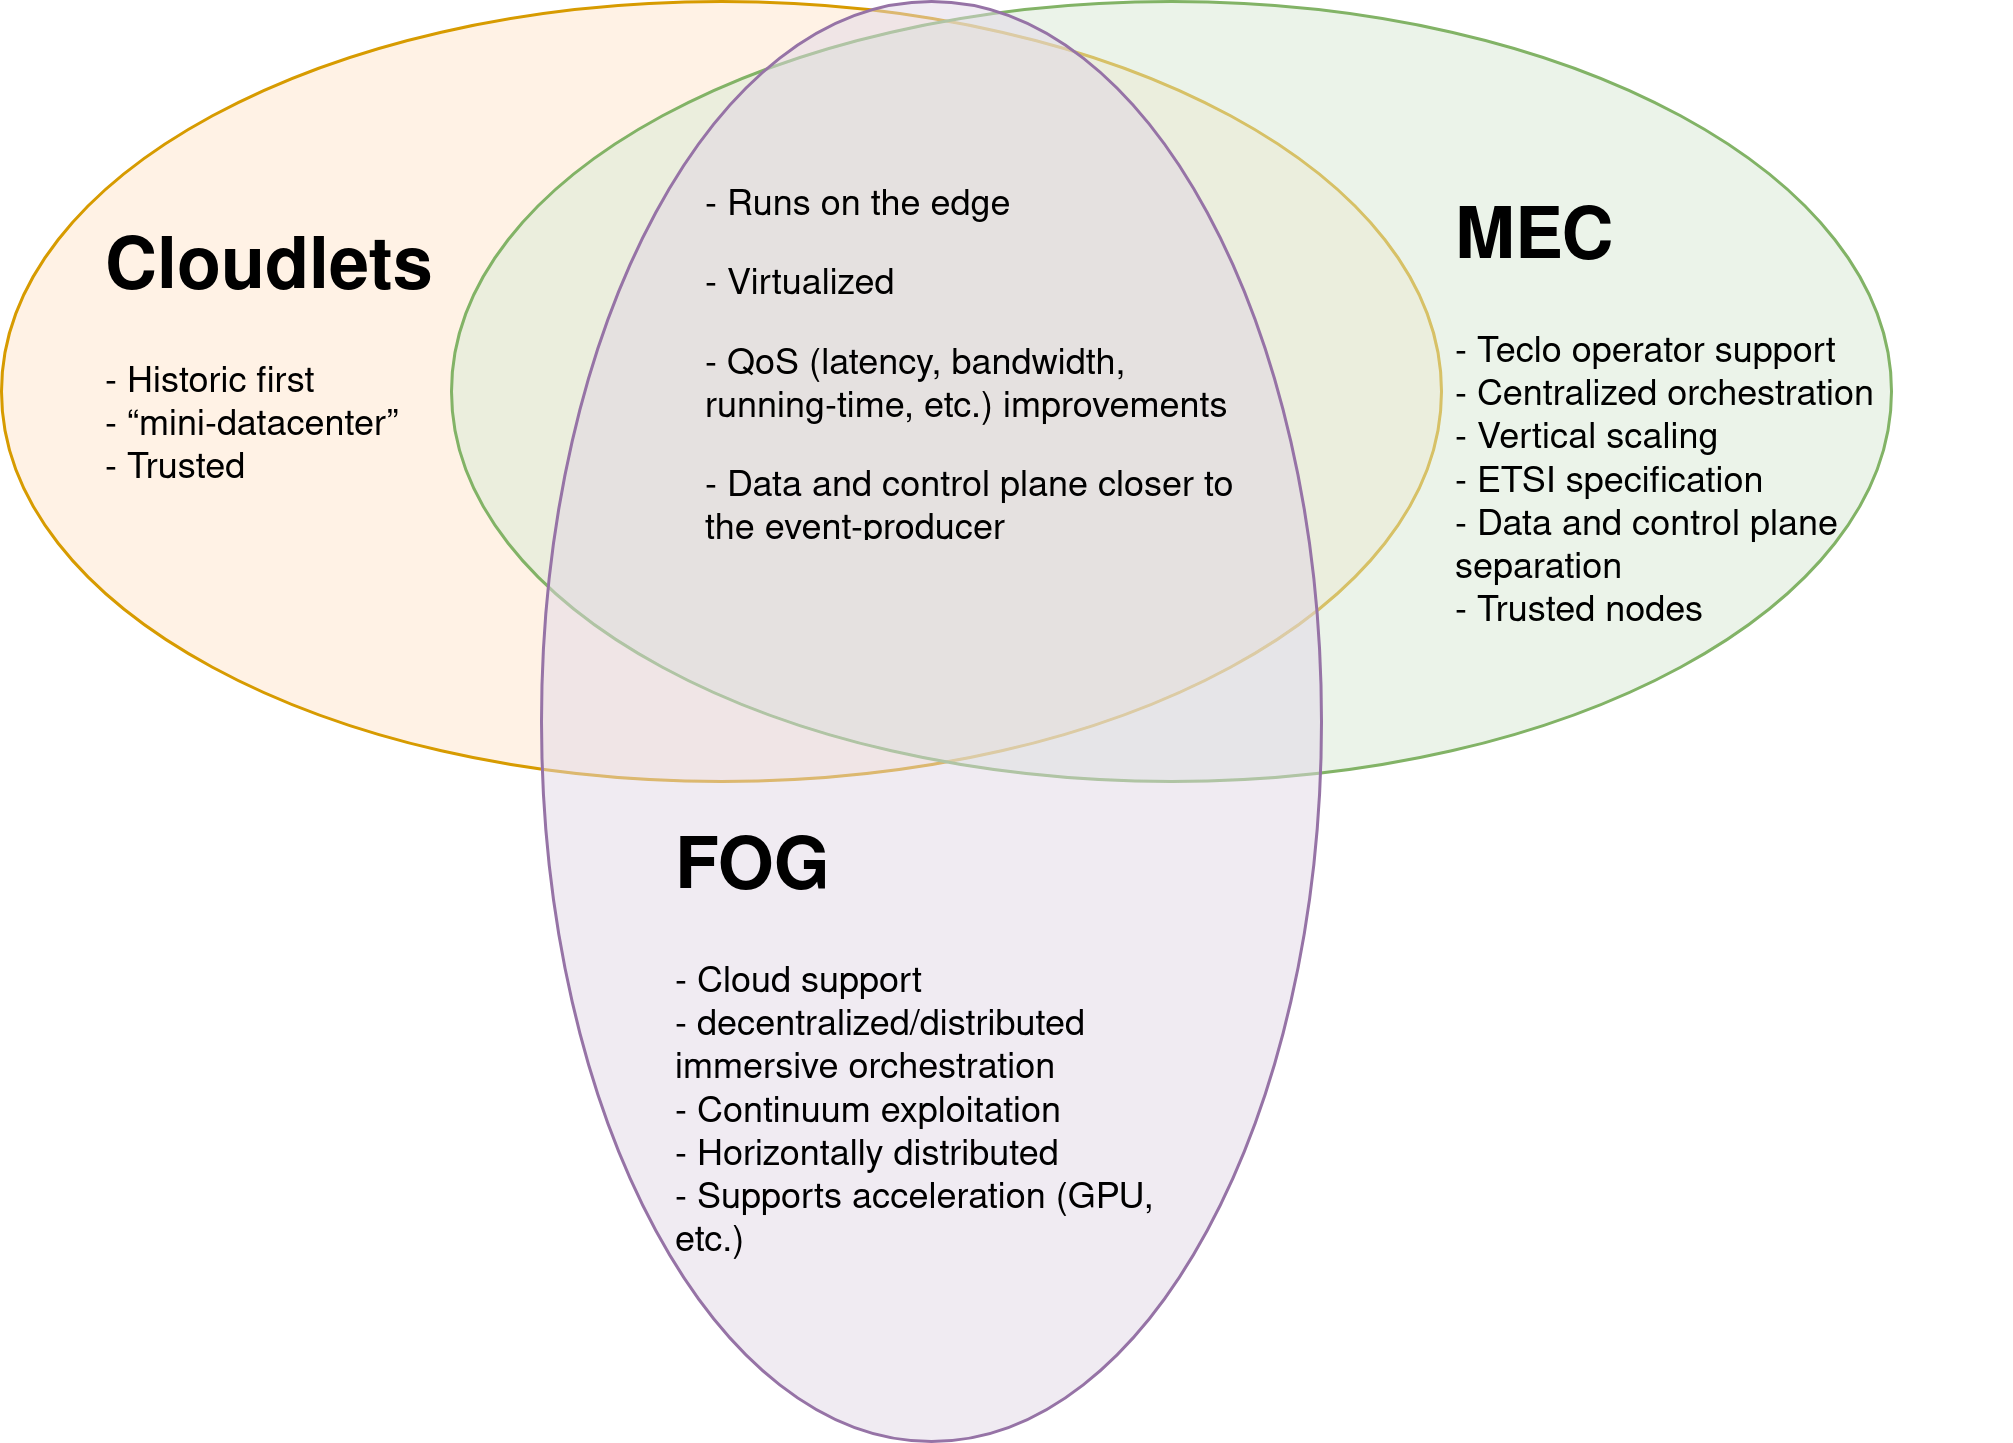
\includegraphics[width=0.75\textwidth]{./assets/CloudLetsVMECvFog.drawio.png}
	\caption{Key differences between all the edge -- and beyond -- paradigms}
	\label{fig:fogVall}
\end{figure}

While all these concepts focus on exploiting the edge of the networks to achieve similar goals constrained by similar challenges, only Fog exploits all the continuum and considers Cloud as much as the edge -- and further than it. Another point highlighted here is the historical progression of ideas, starting with the cloudlets up to a totally distributed paradigm that is Fog computing. However, only \gls{MEC} posses a specification as of 2022. The Fog Continuum acknowledges it and recommend the Fog initiative to avoid duplication of efforts and focus on aspect not optimized by other approaches such as \gls{MEC}. In the long term, it hopes liaisons will form to bring the industry to a common ground \cite{ieee_standards_association_ieee_2018}. The key differences are highlighted in  figure\ref{fig:fogVall}.

\subsection {Context}
\begin{itemize}
	\item introduce serverless in more depth
	\item Introduce \gls{FaaS}
	\item About serverless, \citeposs{elgamal_costless_2018} work about AWS Greengrass shed the light on the ability to maintain serverless applications under a certain latency threshold by utilizing a fusion-placement algorithm that finds non-trivial memory and placement configurations.
\end{itemize}

\subsection {Applications}
\begin{itemize}
	\item No large-scale general-prupose Fog platform is currently publicly available \cite{ahmed_fog_2019}
	\item Yet to have one to exploit, developers should be aware of the firsts applications that can be taken into account
	\item Fog is envisioned to be efficient in terms of bandwidth usage, performance and latency
\end{itemize}
\begin{itemize}
    \item Vehicules
    \item \gls{AI}
\end{itemize}

\section{Platforms}

A variety of platforms exist to accommodate Fog with the current state of industrial applications. Most of them are focused on a private usage. The node is owned by only one user that exploit a small park of nodes for his only benefit. However, many options -- especially the \gls{OSS} ones -- offer the feature of modification and extension needed to bring the Fog paradigm to the next step. For now, most of these platforms are derivative of successful Cloud-based ones, this state-of-the-art leads to technical challenges of running this kind of platform in a resource-constrained fog node.
During this internship, the light will be shed on \gls{OSS} platforms, as they are easier to use, have a public community and documentation linked to the underlying code, and are the only option compatible with open/reproducible research \cite{kjorveziroski_iot_2021}.

%\begin{itemize}
%    \item Several choices
%    \item Main question is to either use already developed code to adapt to the Fog, or to create a new interoperable platform
%    \item The focus is on adaptability, as Fog encompass and extends Cloud
%    \item The technical problem is then to adapt the technology for a new, more demanding platform.
%    \item a distinction can be made between commercial extension and \gls{OSS} extension. The later one can mitigate the vendor lock-in problem described by \citet{kjorveziroski_iot_2021}, and if not, is the only category compatible with open/reproducible research.
%\end{itemize}

\subsection{Commercial focus}

These proprietary platforms are published by cloud giants. The list include, but is not limited to Amazon AWS Greengrass \cite{noauthor_aws_nodate}, Microsoft Azure IoT edge \cite{noauthor_iot_nodate} and Google Iot core \cite{noauthor_cloud_nodate}. Usually these platforms connect to their editor's cloud as another premium service offered from their panel. The use is then exclusive to the developer connecting them. The functionalities offered can be close to \gls{FaaS}, but triggered and processed closer to the data source \cite{elgamal_costless_2018}.

%\begin{itemize}
%    \item Existing offers from cloud giants, such as  \citeposs{elgamal_costless_2018} work emphasize on cost optimization of serverless computations spanning from the cloud to the very edge where Greengrass can be executed on a node by a user. Though the authors use what they called an edge node, it actually corresponds to the characteritics of a fog node placed at the edge of their network.
%    
%    %Durable functions = Greengrass for microsoft, Azure IoT edge ?
%\end{itemize}

\hypersetup{linkcolor=}
\subsection{\acrfull{OSS}}
More transparent platforms are available, this is especially true for \gls{OSS} projects such as Apache OpenWhisk \cite{noauthor_apache_nodate}. It has been started by IBM and then made publicly available through an Apache 2.0 license. This kind of platform is preferred in the era of open-research for obvious reasons as well as limiting an existing Cloud problem: vendor lock-in \cite{kjorveziroski_iot_2021}. Adaptations have been made to retain the benefit of the source code while running on the more resource-constrained Fog nodes. The project is named Lean OpenWhisk \cite{breitgand_lean_2018}.

Another axis of development is focused on a variety of Kubernetes extensions \cite{bocci_secure_2021}, to name a few
\begin{enumerate*}[(a)]
\item Fission
\item Kubeless
\item Knative
\item OpenFaaS
\item Nuclio
\end{enumerate*}.

Other works have focused on the opposite problem. Instead of adapting the Cloud paradigm to the Edge, edge-native platforms have started to appear. \citet{pfandzelter_tinyfaas_2020}] shows better performances than Lean OpenWhisk. While the work is impressive, could it ever reach the industrial development level of platforms such as OpenWhisk once their complete adaption will be achieved? \citeposs{george_nanolambda_2020}'s NanoLambda is another mighty small platform placed at the edge. Thought not compared, it would extend the reach of Fog to Clusters of IoT devices by making devices such as Espressif's ESP8266 \gls{SoC} \cite{noauthor_esp8266_nodate} able to run \gls{FaaS} platforms. Thus enabling a closer layer of processing right inside IoT networks.


\section{Placement}

\newcommand{\tabred}{-4pt}
\newcommand*\rot{\rotatebox[x=2cm]{90}}
\begin{landscape}
\begin{longtable}{
    | l<{\hspace{\tabred}} 
    | >{\hspace{\tabred}}c<{\hspace{\tabred}} 
    | >{\hspace{\tabred}}c<{\hspace{\tabred}} 
    | >{\hspace{\tabred}}c<{\hspace{\tabred}} 
    | >{\hspace{\tabred}}c<{\hspace{\tabred}} 
    | >{\hspace{\tabred}}c<{\hspace{\tabred}} 
    | >{\hspace{\tabred}}c<{\hspace{\tabred}}
    | >{\hspace{\tabred}}c<{\hspace{\tabred}}
    | >{\hspace{\tabred}}c<{\hspace{\tabred}}
    | >{\hspace{\tabred}}c<{\hspace{\tabred}}
    |}

\hline

\diagbox[dir=NW]{\rule{0mm}{4.2cm}\rule{0.9cm}{0cm}Article}{Feature}
& \rot{Centralization} % 1
& \rot{Control level} % 2
& \rot{Isolation mechanism} % 3
& \rot{Placement optimization goals} % 4
& \rot{Allocation mechanisms} % 5
& \rot{Scheduling metrics} % 6
& \rot{SLA or SLO support} % 7
& \rot{Ownership} % 8
& \rot{Security}\\

%\midrule
\hline

\citet{cheng_fog_2019}
& Centralized
& Functions and data
& Containers
& Data centric programming model
& data flow optimality
&  data i/o, geoscope, priority, SLA
& SLO
& total  
& -
\\
\citet{baresi_paps_2019}, \cite{baresi_towards_2019, baresi_paps_2021}  
& Decentralized    
& Functions    
& Containers    
& latency    
& multilayered, with a leader at each step    
& Inter-node latency, network topology, response time, availability, workload, clients, geo-location   
& SLA  \& SLO    
& total   
& - 
\\
\citet{lee_trustful_2020}  
& Decentralized    
& Resource-level provisioning    
& -    
& minimizes use of computational resources    
& maximization of the utility/profit    
& one-shot \acrshort{VCG}   
& -    
& -   
& blockchain to trace transactions 
\\
\citet{cicconetti_decentralized_2021}  
& Decentralized    
& Function    
& -    
& response-time    
& routing algorithm    
& network congestion, response-time   
& -    
& $1-*$   
& -
\\
\citet{wang_lass_2021}  
& Federated 
& resource provisioning   
& containers    
& latency    
& provisionning, deflation   
& SLO  
& -    
& -  
\\
\citet{tasiopoulos_fogspot_2019} 
& decentralized    
& allocation or not    
& VM    
& Revenue or highest possible volume of requests    
& Real-time Dutch auctions   
& -  
& multiple    
& - 
\\
\citet{mutichiro_qos-based_2021} and \cite{palade_swarm-based_2020}
& Federated    
& Functions    
& containers
& Ant Colony Optimization    
& node (CPU, RAM) utilization, service-time, scheduling cost   
& -  
& -
& -  
\\
\hline
\end{longtable}
\end{landscape}




\subsection{Literature review}

As previously introduced, the novelty of Fog research makes it hard to compare the landscape. To fix such a problem, surveys are conduced, such as \citeposs{bocci_secure_2021}. 

%They introduce \cite{cheng_fog_2019, baresi_paps_2019, baresi_towards_2019, cicconetti_decentralized_2021}\\ % mortzavi + perssons

\begin{description}
	\item[\citet{cheng_fog_2019}] defines \textit{Fog functions} as a new \gls{FaaS} platform. They note data locality is of ``paramount'' importance. Data are observed to be linked with variable
	\begin{enumerate*}
		\item entity size
		\item entity refresh rate
		\item task complexity
		\item task running-time
		\item task priority
		\item task novelty
	\end{enumerate*}. The authors also identify what a data-intensive Fog framework should provide: 
	\begin{enumerate*}
		\item data discovery and routing fine-grained to the content of the data
		\item function triggering solely based on the availability of the input data
		\item dynamic placement of either data or code to the best processing place
		\item data dependency as function composition driver
	\end{enumerate*}.
	Nodes are edge-base or cloud-based and running the same software. Discovery and orchestration is centralized onto a particular node. The orchestrator is aware of data flowing to its nodes. It then decides where to execute each function. Data is then routed to that node and processing takes place.
	
	\item[\citeposs{baresi_paps_2019}] \gls{FaaS} platform is focused on low-latency, data-intensive use cases. \cite{baresi_towards_2019} identify multiple challenges to the creation of a \gls{MEC} platform by the research community, it comprises
	\begin{enumerate*}
		\item resource management
		\item placement \& migration of application components and services between platforms
		\item scheduling of computation and offloading from mobile and \gls{IoT} devices
	\end{enumerate*}. The authors also notes a Fog platform is not yet extensively understood and defined.
	The paper defines a \gls{SEP} that answers a list of requirements:
	\begin{enumerate*}
		\item low-latency computation offloading
		\item inter-platform collaboration to ensure \gls{SLA} deadlines
		\item latency optimization to enable real-time communications
		\item opportunistic data analysis for anticipation
		\item edge coordination to enforce location awareness
		\item Stateful partitions to extend \gls{FaaS} support
	\end{enumerate*}.
	The authors then proceed to create a prototype implementing each of those points. Their solution is deployed on OpenWhisk. They observe a need to reduce latency, especially in real-time scenarii.
	
	\citet{baresi_paps_2019, baresi_paps_2021} extend this work with the \gls{PAPS} platform while advocating for a decentralized approach, effectively reducing speed of control.
	The architecture is divided into 3 layers:
	\begin{enumerate*}
		\item A supervisor node that knows the global topology. Its responsibility is to form communities
		\item A community is an aggregation of nodes having a common reduced communication delay (under a defined threshold). It has been assembled by the Supervisor node and is in charge of making sure \glspl{SLO} are reached and \glspl{SLA} not violated. The functions processed by the community are allocated by a leader. This centralized approach avoids the need of a more complex protocol while using well known optimal centralized techniques. The authors note utilizing containers in \gls{PAPS} make reactivity challenging.
		\item The community leader then passes the responsibility to a local node, alongside the allocated resources. Then it is up to that local node to make sure \gls{SLO} is not broken with respect to other executing applications it handles. So each node actually micromanages its allocated functions and their fluctuations the best they can, while still respecting the leader's decision and global view.
	\end{enumerate*}
	
	Following the theory, and after a promising simulation, \citet{baresi_paps_2021} implements \gls{PAPS} on top of Kubernetes and OpenFaaS. Their conclusion is their partitioning allows for guarantees that decentralized heuristics cannot provide, while still doable in practice, unlike a fully centralized architecture. They also point out they can handle highly fluctuating workloads.
	
	\item[\citet{lee_trustful_2020}] position themselves in the \gls{IoV} paradigm, where vehicles interact with \glspl{RSU} located alongside the roads. The authors note in this case the untrustworthy vehicles can be used as attack vectors to compromise both the stability and the data integrity of the service by attacking the trusted \glspl{RSU}. Their contribution is a platform based on allocations decided by a one-shot version of the \gls{VCG} auction scheme named ``the Hungarian method'' \footnote{The ``the Hungarian method'', while ensuring one-to-one assignment of computing resources, finds the lowest cost way to divide the said resources \cite{wikipedia_hungarian_2021}. In \cite{lee_trustful_2020}, minimizing the cost is equivalent to a minimization of utilities, meaning the resources are strictly utilized to the necessary.}. Vehicles are bidding on computing resources made available by the \glspl{RSU}, or their adjacent neighbors. It is optimal for vehicles to bid their true utilities. If they do so, the resource assignment is fair. Results and purchased service times of transactions are secured using a tweaked and distributed blockchain that saves on both energy and computing power. The auction is initiated by the auctioneer -- a \gls{RSU} node -- and is broadcasted back to vehicles by adjacent nodes. Simulation of the platform concludes latency is negligible, while proportional to the number of connected vehicles. The second conclusion is that this method is deemed realizable.
	
	\item[\citet{cicconetti_decentralized_2021}] propose a decentralized platform to minimize response times while respecting short- and long-term fairness in stateless task assignations. Their platform does not extend to the Cloud and integrates by the standards of the \gls{MEC} model. An edge device is connected to an edge router that submits the stateless task request to an edge computer. The router decides autonomously where to forward the task in his known pool of compute-enabled nodes. The router proceeds to
	\begin{enumerate*}[(a)]
		\item update path weights \label{cicconetti_weights}
		\item choose a destination \label{cicconetti_destination}
	\end{enumerate*}.
	\ref{cicconetti_weights} is achieved by measuring a rolling average of routed function response times submitted to computing nodes. A \gls{SDN} controller supervising the network is used to know and avoid congested paths. \ref{cicconetti_destination} has been tested on three different algorithms. Namely 
	\begin{enumerate*}[(i)]
		\item \gls{LI} -- always select the minimum cost node \label{cicconetti_li}
		\item \gls{RP} -- selects a random node with a probability proportional to the weighted \ref{cicconetti_weights} path to that node \label{cicconetti_rp}
		\item \gls{RR} combines the proportional benefits of \ref{cicconetti_rp} with the greediness of \ref{cicconetti_li} \label{cicconetti_rr}
	\end{enumerate*}.
	\ref{cicconetti_rr} achieves both short- and long-term fairness, while \ref{cicconetti_rp} only the latter. \ref{cicconetti_li} is the worst performer.
	The authors conclude the \gls{SDN} plays a capital role in the system. Under load variations, performance is equally as good as in a regular distributed systems. Finally, exploration of hierarchical forwarding in a simulated test-bed with OpenWhisk offers interesting scalability perspectives.
	
	\item[\citeposs{wang_lass_2021}] \gls{LaSS} platform is based on queuing models to manage resources with an exclusive focus on latency sensitive computations in edge clusters. The platform aims at ensuring each function meet its \gls{SLO} deadlines. The platform differentiates two behaviors: the absence of resource pressure and its contrary, alongside overloads. 
	\textcolor{red}{Present what happens in pressure. Forgot to finish reading the article there...}
	Anyway, the platform will monitor its functions in order to balance provisioning between them, allocating reclaimed resources to under-provisioned functions. A prototype of the platform is implemented on top of OpenWhisk to conduct an experimental evaluation. It concludes .
	
	\item[\citeposs{tasiopoulos_fogspot_2019}] FogSpot allows the provisioning of heavily stateful \glspl{LLA} -- \glspl{VM} that can neither be migrated nor suspended -- on Fog nodes along the path of an Edge device's request to its default execution location: the Cloud. That way either the request is accepted and provisioned or, it is forwarded to another further node. If it only gets forwarded, it ends up executed in the Cloud. 
	Each node hosts a trusted market. A \gls{LLA} request is also truthful bid that shows its willingness to pay per unit of time and is directly related to its \gls{QoS} gain that would be observed if the request was to be accepted and the application served on this particular node. Of course, the further the request is from the edge, the lower the bid and the utility gets, until it finally reaches 0 and the Cloud.
	Each node can either choose to maximize its revenue or its social welfare. Those strategies are reflected in the used Dutch auctions termination's conditions. Such auctions are employed to keep processing requests on the spot, without having to queue and to wait anywhere along the request's way. A depth analysis of executions is conducted by the authors and reveal the first strategy leads to more gain for the node's provider but with uncertainties on the prices when executed in a decentralized/uncoordinated way while the second one will try to fully exploit the capacity of the node and provide a stable solution in an uncoordinated space.
	
	\item[\citeposs{mutichiro_qos-based_2021}] contribution is STaSA, a scheduler developed for KubeEdge to be executed in a \gls{MEC} -- a community of Fog Nodes: multiple nodes aggregated around a leader because of their proximity latency-wise, here thought to be in a server rack. The scheduler is introduced as a way to respect as much as possible applications' \gls{QoS} requirements. Other objectives are also considered: node utilization maximization, cost minimization (compared to standard Cloud) and service-time optimizations. This problem is NP-hard. STaSa is built upon the \gls{ACO} probabilistic model to place containers -- called functions throughout the article. The model has been tweaked, especially during the pheromone updates and calculations. In principle, ants are dispatched to the nodes to find the best suitable placement. On their way back they leave a pheromone trace. Its intensity/weight depends on a number of factors the ant found in the node (CPU/RAM utilization, latency, QoS, etc.). Termination is reached when either a threshold is reached or when the best placement is found: when the minimal cost is thought to have been found. Practical implementations showcase better results than baselines \gls{ACO} and First Come First served strategies.
	
	\item[\citet{palade_swarm-based_2020}] can be directly compared to \cite{mutichiro_qos-based_2021}. Noting that the first dates back to \citedate{mutichiro_qos-based_2021} whereas the latter is older by a year ( \citedate{palade_swarm-based_2020} ). They both utilize the \gls{ACO} meta-heuristic algorithm. However, \cite{palade_swarm-based_2020} concentrates explicitly on \gls{MEC}. They also succeed to show this approach leads to less overall latency. They argue this gain largely mitigates the failure to find an optimal load-balancing and a ``sub-second'' higher execution time.
	
	
	
	\item[Skippy]
	\item[MPSC]
	\item[Bermbach et al.] with infrastructure PoV
\end{description}


% only request to cloud ? what happens if latency constrained ? Does it have to pay more ? what if load?

% TODO explain \gls{VCG}
% TODO explain blockchain
% TODO explain KubeEdge
% Bulk Synchronous Parallel (BSP) as elaborated in [18] for Faas ?

% another problem : versionning of the nodes and their executed content
% another problem : do we take the user preference, in term of placement, energy (from Ayan Mondal, preprint emailed)

% Explain why Fog placement and FaaS placement cannot be separated from orchestration, because of the impact of each other

% cicconetti_decentralized_2021 has examples for applications + points out the need of a custom platform because of high overhead of K8S, etc.

% decentralized != distributed

% ETSI specifications https://www.etsi.org/technologies/multi-access-edge-computing

%\subsection{Charateristics}
%Introduce to the different hightlighted differences between all the methods
%\begin{itemize}
%    \item centralized vs decentralized
%    \item coarse grained vs fine grained
%    \item isolation mechanism (VM, container, WASM, etc.)
%    \item Placement aim (latency, trhoughtput, cost reduction, redundancy, etc.). What does it optimize?
%    \item Allocation mechanism (fair, always a wninner, utility optimization, auctions, etc.)
%    \item Used metrics for scheduling
%    \item SLA support, or any kind of agreements
%    \item Multi landlord environement?
%    \item Security, cf Figure 16 of \citeposs{ieee_standards_association_ieee_2018} openfog standard
%\end{itemize}
%\begin{itemize}
%    \item Usually more popupar in the litterature
%    \item Simplifies the problem by considering the infrastructure owned by the same actor
%    \item Simplifies the layered model: Cloud, then Edge often as a horizontal layer
%    \item Was developed and advertised before the Fog
%    
%\end{itemize}
%
%
%Usually these approach rely on a scheduler mastering a subset or the whole node network. This is the approach that is the most optimal as the master knows the whole state of the system
%\begin{itemize}
%    \item matrix chain ordering problem \citet{elgamal_droplet_2018}
%    \item \citeposs{palade_swarm-based_2020} defines Multi-acccess Edge Computing. A server acts as an intermediary between the cloud and other sub-nodes. This is a sort of master of the underlying network. The scheduler is cloud based.
%\end{itemize}
%
%\begin{itemize}
%    \item \citeposs{wang_lass_2021} Developped a platform that uses fair share allocation mechanisms. This guarantees a minimum allocated resources to each function, in case of an overload of the node. Their platform is recommended by the authors for highly dynamic predictible workloads as it utilizes aggressive approaches to reclaim resources at the scale of hundreds of milliseconds. Sadly, this approach is tested for the edge, with more computing power than in fog. Another critic is that it only focuses on a single node.
%    \item Not all papers are about managing the behaviours of the Fog, some focus on optimization of the execution of the functions themselves, such approches are explored by \citet{shen_defuse_2021} that utilizes mining pattern to extract execution dependencies, thus optimizing along the way.
%\end{itemize}
%\begin{itemize}
%    \item \citeposs{mutichiro_qos-based_2021} tested an approched focuses solely on QoS optimization
%\end{itemize}
%
%\begin{itemize}
%    \item \citet{lee_trustful_2020} utilizes VCG auctions to allocate computing resources. The transactions are secured using blockchain contracts. The paper is only about a simulation as a proof of feasability and lacks proper load verification.
%    \item {Approach of blockchain, w/ replacement of the Proof-of-Work with something lighter, as highlighted by \citet{xie_when_2021} in their survey of applied auctions an blockchained. \begin{enumerate}
%        \item \citet{zavodovski_decloud_2019} created a distributed auction platform
%        \item \citet{debe_blockchain-based_2020} explores reverse bidding
%        \item \citet{yu_building_2019} makes sure to find a winner in the edge nodes for every requests submitted
%        \item There are also mentions about deep learning-based auctions, that are optimal
%        \item \citeposs{mutichiro_qos-based_2021} tested an approched focuses solely on QoS optimization
%    \end{enumerate} }
%\end{itemize}
%
%%\subsection{Centralized vs Decentralized}
%%\subsubsection{Centralized}
%%\begin{itemize}
%%    \item \citet{cheng_fog_2019} defines \textit{Fog functions} as a \gls{FaaS} platform. Nodes are edge-base or cloud-based and running the same software. Discovery and orchestration is centralized to a particular node. The orchestrator is made aware of the data flowing to its nodes. It then decides where to execute the function. Data is then sent to that node so processing can take place.
%%\end{itemize}
%%
%%\subsubsection{Decentralized}
%%\begin{itemize}
%%    \item{ \citet{baresi_towards_2019} theorised an edge-only platform that would collaborate with others. Their goal is to optimize latency and trhoughtputs of the applications they execute. Their platform would both be able to orchestrate the swarm vertically and horizontally, the later one being prioritized to maximize robustness and availability. \citeposs{baresi_paps_2019} \gls{PAPS} automatic platform is an application of their principles, at a superiror scales from their perspective. They can execute 100 functions on an intense workload. The platform divides itself into 3 layers.
%%    \begin{enumerate*}
%%        \item A supervisor node that knows the global topology. Its responsability is to form communities
%%        \item A community is an aggregation of nodes with a reduced communication delay (under a defined threshold). It has been assembled by the Supervisor node and is in charge of making sure \glspl{SLO} are reached and \glspl{SLA} not violated. The functions processed by the community are allocated by a leader. This centralized approach avoids the need of a more complex protocol while using well known optimal centralized techniques. The authors note the utilization of containers in \gls{PAPS} make reactivity challenging.
%%        \item The community leader passes the responsabilty to the local node, alongside the allocated resources. Then it is up to that local node to make sure \gls{SLO} is not broken. So each node actually micro-manage its allocated functions and their fluctuations the best they can, while still respectinf the leader's decision and global view.
%%    \end{enumerate*}
%%    }
%%\end{itemize}
%
%\subsection{Control level}
%
%\subsection{Isolation mechanism}
%%\begin{itemize}
%%    \item \cite{cheng_fog_2019} uses Docker to isolate each functions.
%%\end{itemize}
%
%\subsection{Placement optimization goal}
%%\begin{itemize}
%%    \item \cite{cheng_fog_2019} tries to respect \gls{SLO} at runtime
%%\end{itemize}
%
%\subsection{Allocation mechanism}
%\subsection{Scheduling underlaying metrics}
%
%\hypersetup{linkcolor=}
%\subsection{\acrfull{SLA} support}
%A \acrfull{SLA} is an agreement between the cloud provider and the client specifying uptimes, responsiveness, performance-level, issue resolution timeframe \cite{wikipedia_service-level_2021}. In short what the client expects from what the provider advertised. This cloud native contract would provide a well-known framework to define what to expect from a Fog network. Because Fog is decentralized, one would however need to leverage the correct toolset to make the contract known by all. Such a mechanism can be contributed by smart contracts \cite{hang_sla-based_2019, di_pascale_smart_2017, zhou_trustworthy_2018}.
%\subsection{Ownership: living in a multi landlord ecosystem}
%\subsection{Security}
%\subsubsection{Physical attacks}
%Compromised hardware can be a possibility, however harming the provider.
%\subsubsection{Anything else}
%Other risks are known, from exploitation of resource contrained policies to more problematic auxilary attacks. To not over-extend this research domain, Fog computing would only worsen issues such as coverting attacks as desmonstrated by \citet{maurice_hello_2017}. If before the cloud provider was in charge of the virtual machine distribution to a certain extent, Fog introduces geographic constraints. Those would theoretically enable geographically-located attacks.
%This is a critical aspect as \citet{ieee_standards_association_ieee_2018} also points out.

\section{Curated list of unresolved problems}
\begin{itemize}
    \item What did we just learn?
    \item Focus on some of the issues yet to solve
    \item Where are we going? (no papers that go there, yet...)
\end{itemize}

\section{Conclusion}

\printbibliography 

\end{document}
%%% Local Variables:
%%% mode: latex
%%% TeX-master: t
%%% End:
